\chapter{Testing}
At first time running the algorithm, the input vision for the ball to the wave, was from the centre of ball to both sides of the wave as a one point. That made it hard for the ball to find its way (or have a futuristic vision you can say). There would be a change in the wave curve and the ball can't detect it, so an idea came of having more range for the ball to see. It would calculate the distance between the ball rectangle to the left or right side of wave in more than one point.

To get more into it with numbers, there would be a notice of the ball having a weird sense of getting to know its "new" sense of wider vision diameter. The ball would take about 20 generations just to start moving in more random left and right. This is made when the ball had only the vision of its 24-pixel diameter (12px as radius) then extra step of plus 50 pixels, getting this info in nutshell
\begin{itemize}
	\item One point vision: good as start and better CPU wise.
	\item Diameter vision + 20: best one in score yet (117 points in generation 89).
	\item Diameter +50 points: No learning even after nearly 300 generation.
\end{itemize}

The reason to increase the vision for the ball (even though it was working fine) is I wanted to test how long would it take from the ball to get used to the new (increased) amount of lines. I can tell you it took long long enough.

\begin{figure}[H]
	\centering
	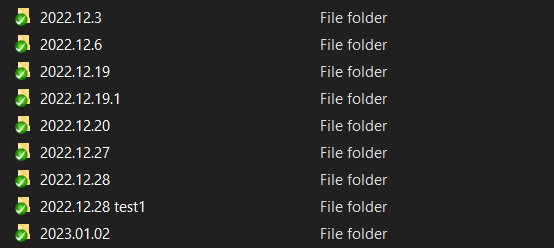
\includegraphics[width=0.7\linewidth]{usedImages/numTrainingSessions}
	\caption[]{Number of training sessions}
	\label{fig:numtrainingsessions}
\end{figure}


At this point of the game, I implemented the increased speed of wave *4 that improved the learning speed. With normal fps, it would take 8 hours 15 min for 37 generation, but the new one (with limitation to 4 times speed, not more) takes 5 hours 15 second for 100 generation to work. That is 4 times the normal running time of normal pace of game for a human to play it, and the generation threshold to be 300 generation instead of 100, let the laptop run as much as it needs. It took more than 15 hours to finish 294 generation and 11 genome, when went back to check the log, none of them managed to pass 3000 fitness score. That means that none of them had a good intuition of the lines to move left or right and at least overcome one curve in the wave. From this, the amount of numbers increased = more time in training.

There is a small box that is shown around the ball, it is called ballRect and mentioned a lot in the \hyperref[sec:count-distance]{Count Distance} and \hyperref[sec:collision]{Collision}. ballRect is shown to check if the genome did terminate for an actual collision or because it reached the threshold, like the case here in this video.

In order to save as much as CPU power during the learning process, the box is shown only when fitness is over 50. In addition to some extra visuals in the game, such as the particles behind the ball, but all of them can be viewed again with a key for each one:
\begin{itemize}
	\item \inlineCode{v Key} to shown \textbf{v}ision
	\item \inlineCode{b key} to show the \textbf{b}allRect
	\item \inlineCode{p key} to show the \textbf{p}articles
\end{itemize}